\newdate{date}{21}{09}{2022}
\date{\displaydate{date}}
\author{Dustin J. Trujillo}

\maketitle

%%\begin{abstract}
%%To be added later.
%%\end{abstract}

\section{Introduction}

My name is Dustin Trujillo and I am a second year PhD student in the Security program, advised by Dr. Li. The skills I have gained through my academic studies and 15 years working full-time in the information technology and information security fields have ultimately let me to pursue a PhD in security out of sheer passion for the field and a desire to contribute to it.

I have a diverse working background in project management, military intelligence, cyber threat intelligence, ethical hacking, malware reversal, network security, and designing and implementing secure on-premise and cloud solutions. However, my primary goals for this PhD program and research are to contribute something new and interesting, and of course, useful, to the field of Information and Cybersecurity, specifically in the subset field of Denial of Service (DoS).

While I am still narrowing down (with Dr. Li) my specific dissertation research proposal, I do get excited about topics like network security/threat hunting/ethical hacking/malware reversal. My goal for this class is to completely narrow down my research topic (which is currently Denial of Service) and have my dissertation proposal completed and ready to be presented to the PhD program committee by the end of this 2022 fall semester.

As far as a few personal items, I love to ski and be outdoors, and my wife and I have 5 kids (blended family) with one on the way! See Figure 1 for a picture of myself.

\begin{figure}[H]
\centering
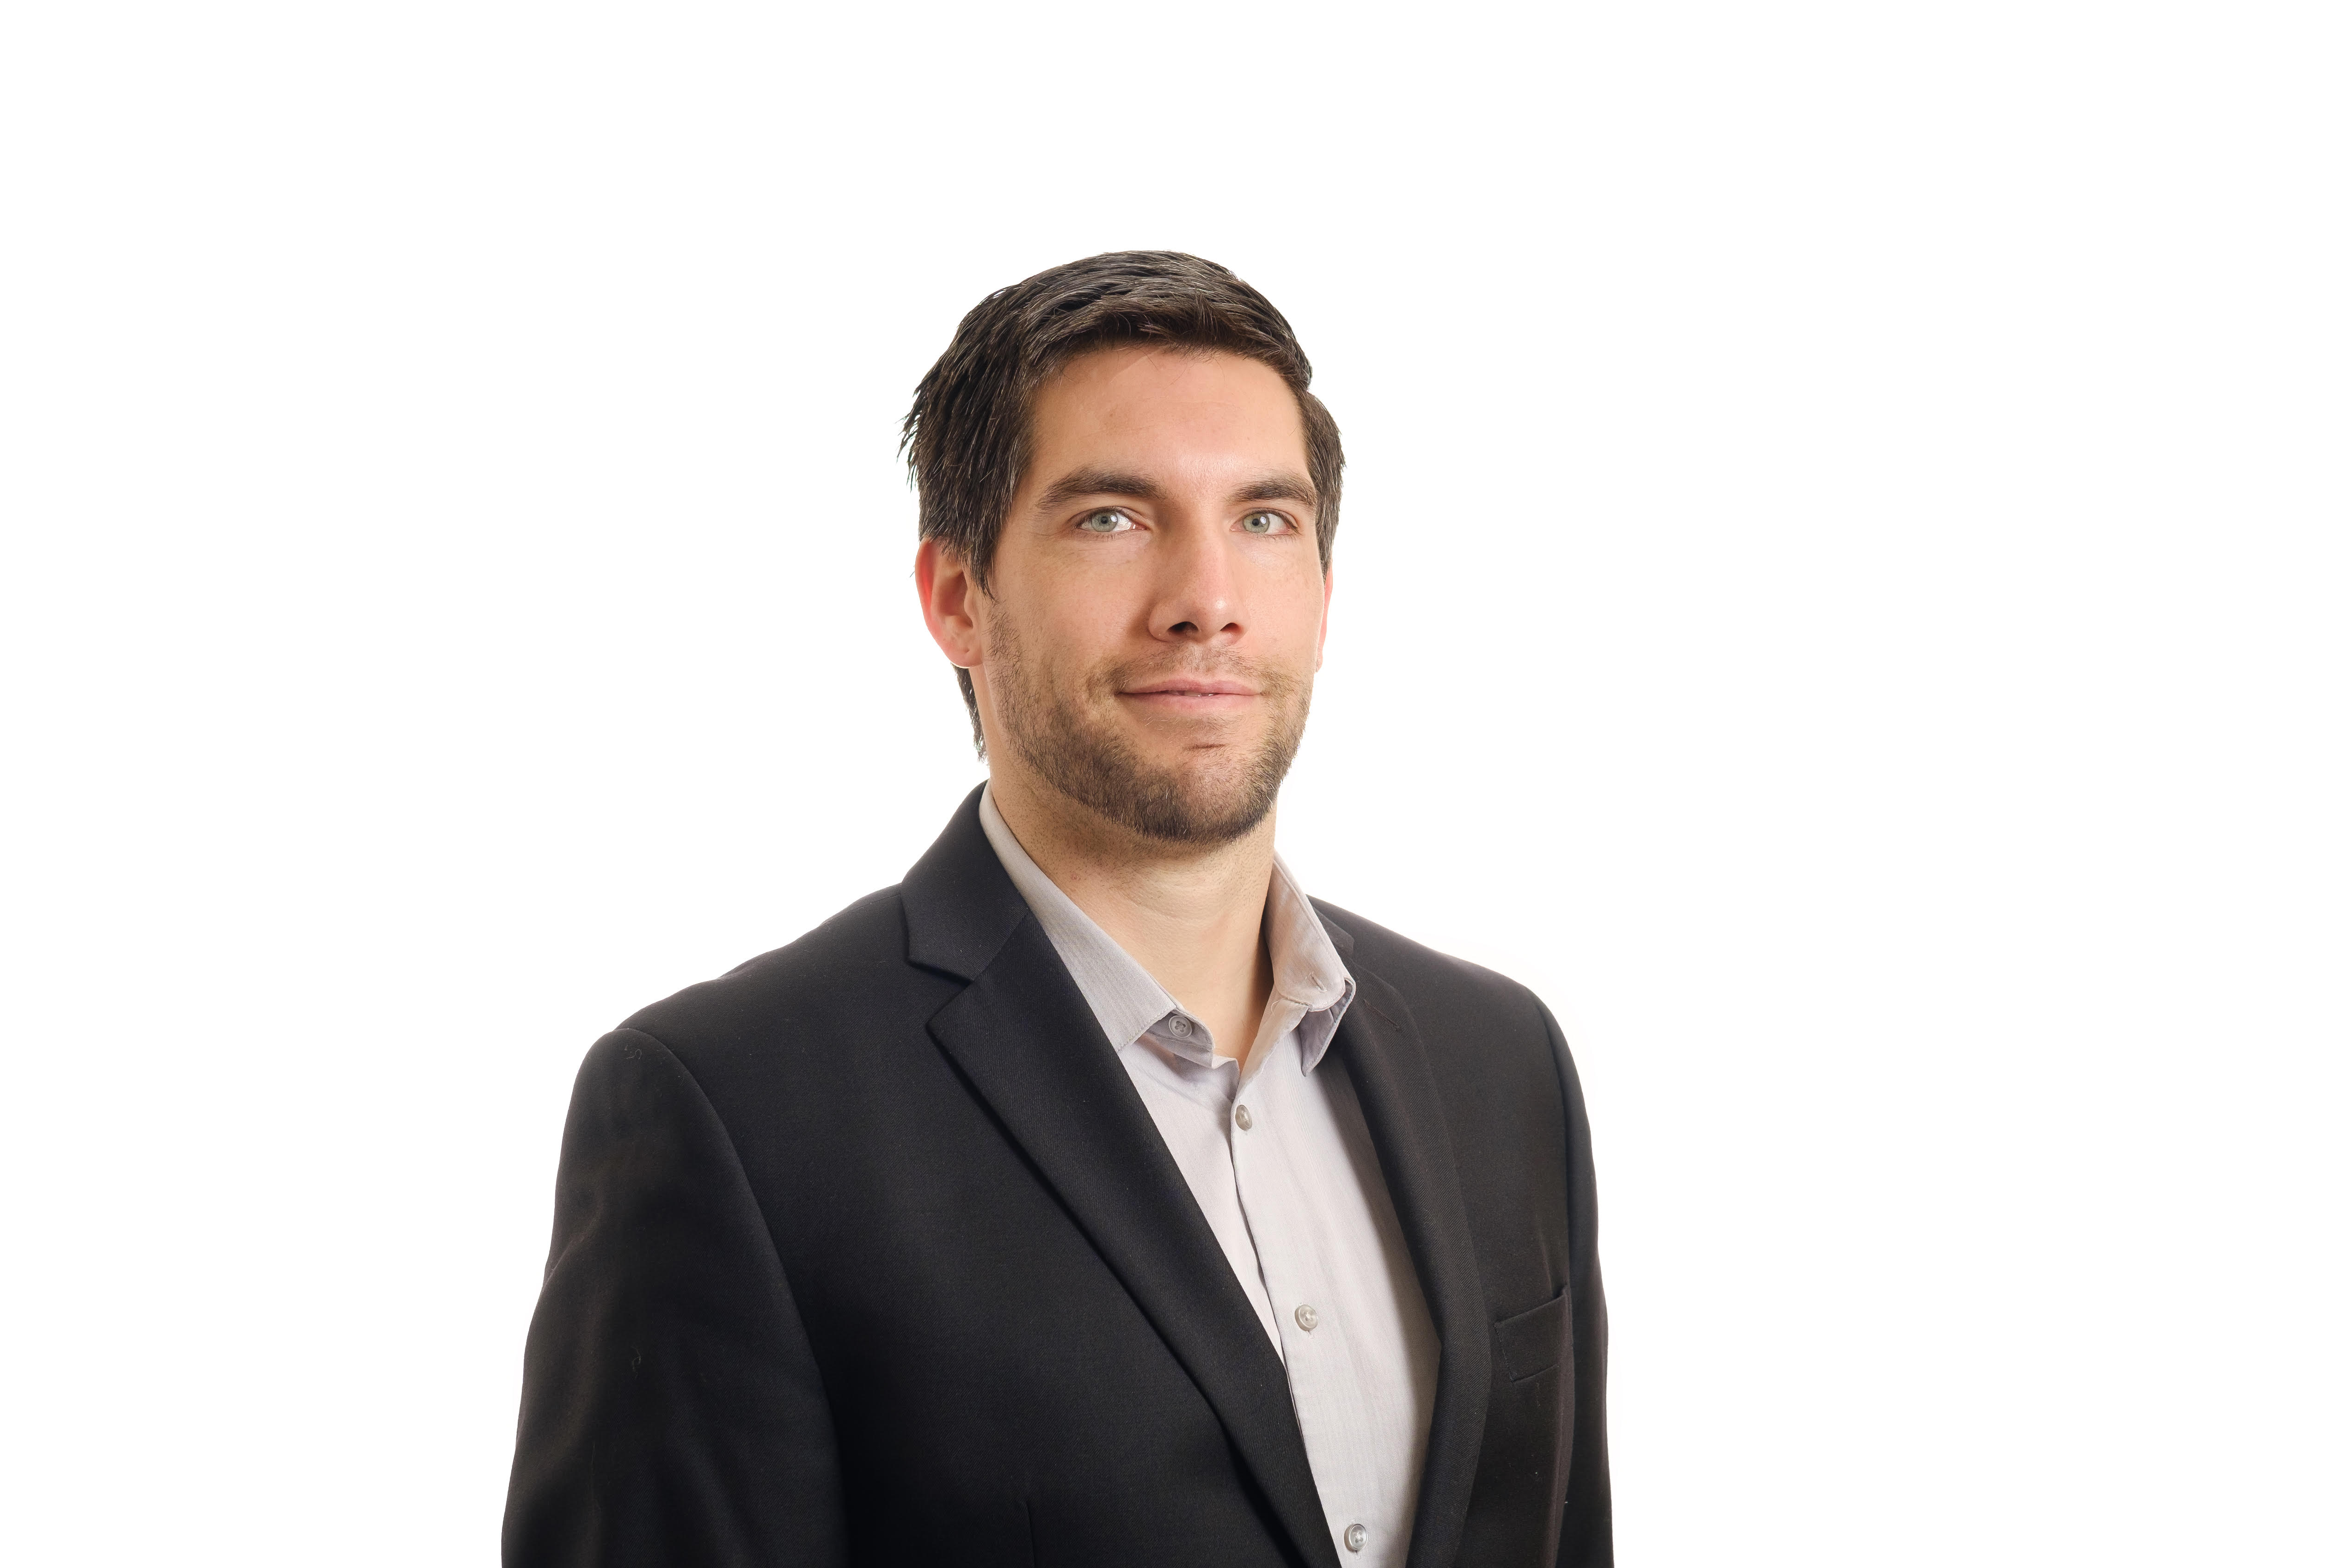
\includegraphics[width=0.3\textwidth]{trujillo.jpg}
\caption{\label{fig:Me}This is a picture of myself.}
\end{figure}


\section{Data on GitHub}
This \href{https://github.com/vz-risk/VCDB}{VCDB: VERIS Community Database} Git repo has code related to my Denial of Service research area. This repo is the VERIS Community Database and includes a lot of data related to data breaches over the past many years. It is the data source that Verizon uses to test/prove/disapprove their assumptions while developing their annual Data Breach report.

\section{Questions To Answer}
1. Q: Hi Dustin, what is the sub-field of cybersecurity you find most interesting?
\\
A: Hi, thank you for asking. I am most intersted in Ethical hacking/Denial of Service. - Dustin Trujillo
\\
2. Q: Dustin, I see you have a diverse background in the cyber realm, do you have certs for some of the background work you have done?
\\
A: Hi, thank you for asking. Yes I do. I have the Security+, C|EH, C|ND, CISSP, and AWS Architect with Security certifications. - Dustin Trujillo
